\chapter{อุปกรณ์ต้นแบบและการแสดงผลบนหน้าจอ}



\section{รูปอุปกรณ์ที่ใช้ในการตรวจจับภาพใบหน้าและรับคำสั่งยืนยัน}

\begin{figure}[!ht]
  \begin{center}
    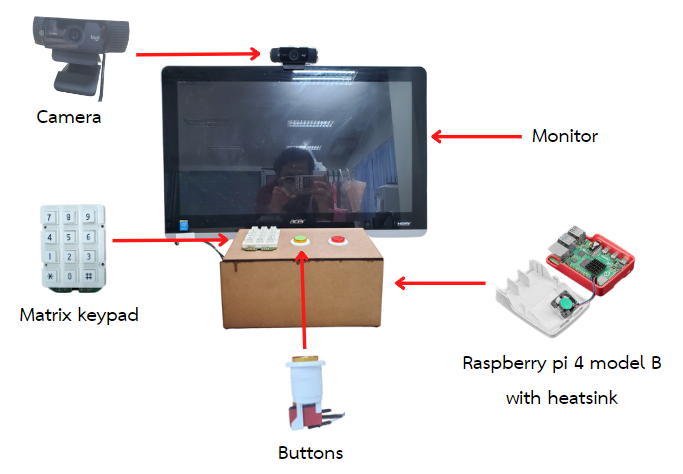
\includegraphics[scale=.6]{pic/overall_module.png}
    \caption[อุปกรณ์ตรวจจับใบหน้า แสดงผลและรับผล]{อุปกรณ์ตรวจจับใบหน้า แสดงผลและรับผล}
    \label{fig:module_pi}
  \end{center}
\end{figure}



% Text for a section in the first appendix goes here.

% test ทดสอบฟอนต์ serif ภาษาไทย
\begin{figure}[!ht]
  \begin{center}
    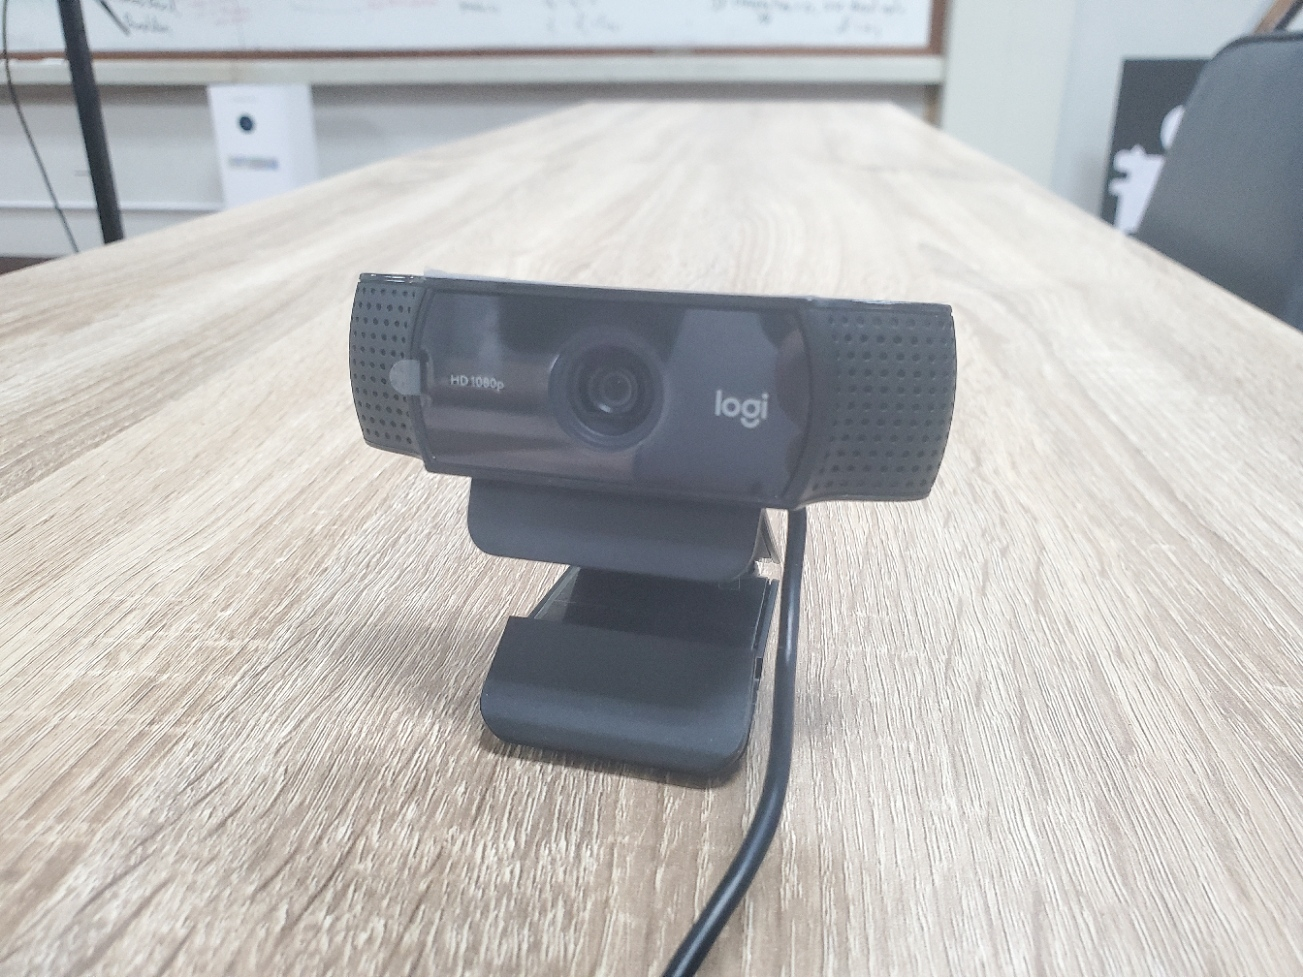
\includegraphics[scale=.15]{pic/camera.jpg}
    \caption[กล้องที่ใช้ในการตรวจจับใบหน้าบุคคล]{กล้องที่ใช้ในการตรวจจับใบหน้าบุคคล}
    \label{fig:camera_logi}
  \end{center}
\end{figure}

% \begin{figure}[!ht]
%   \begin{center}
%     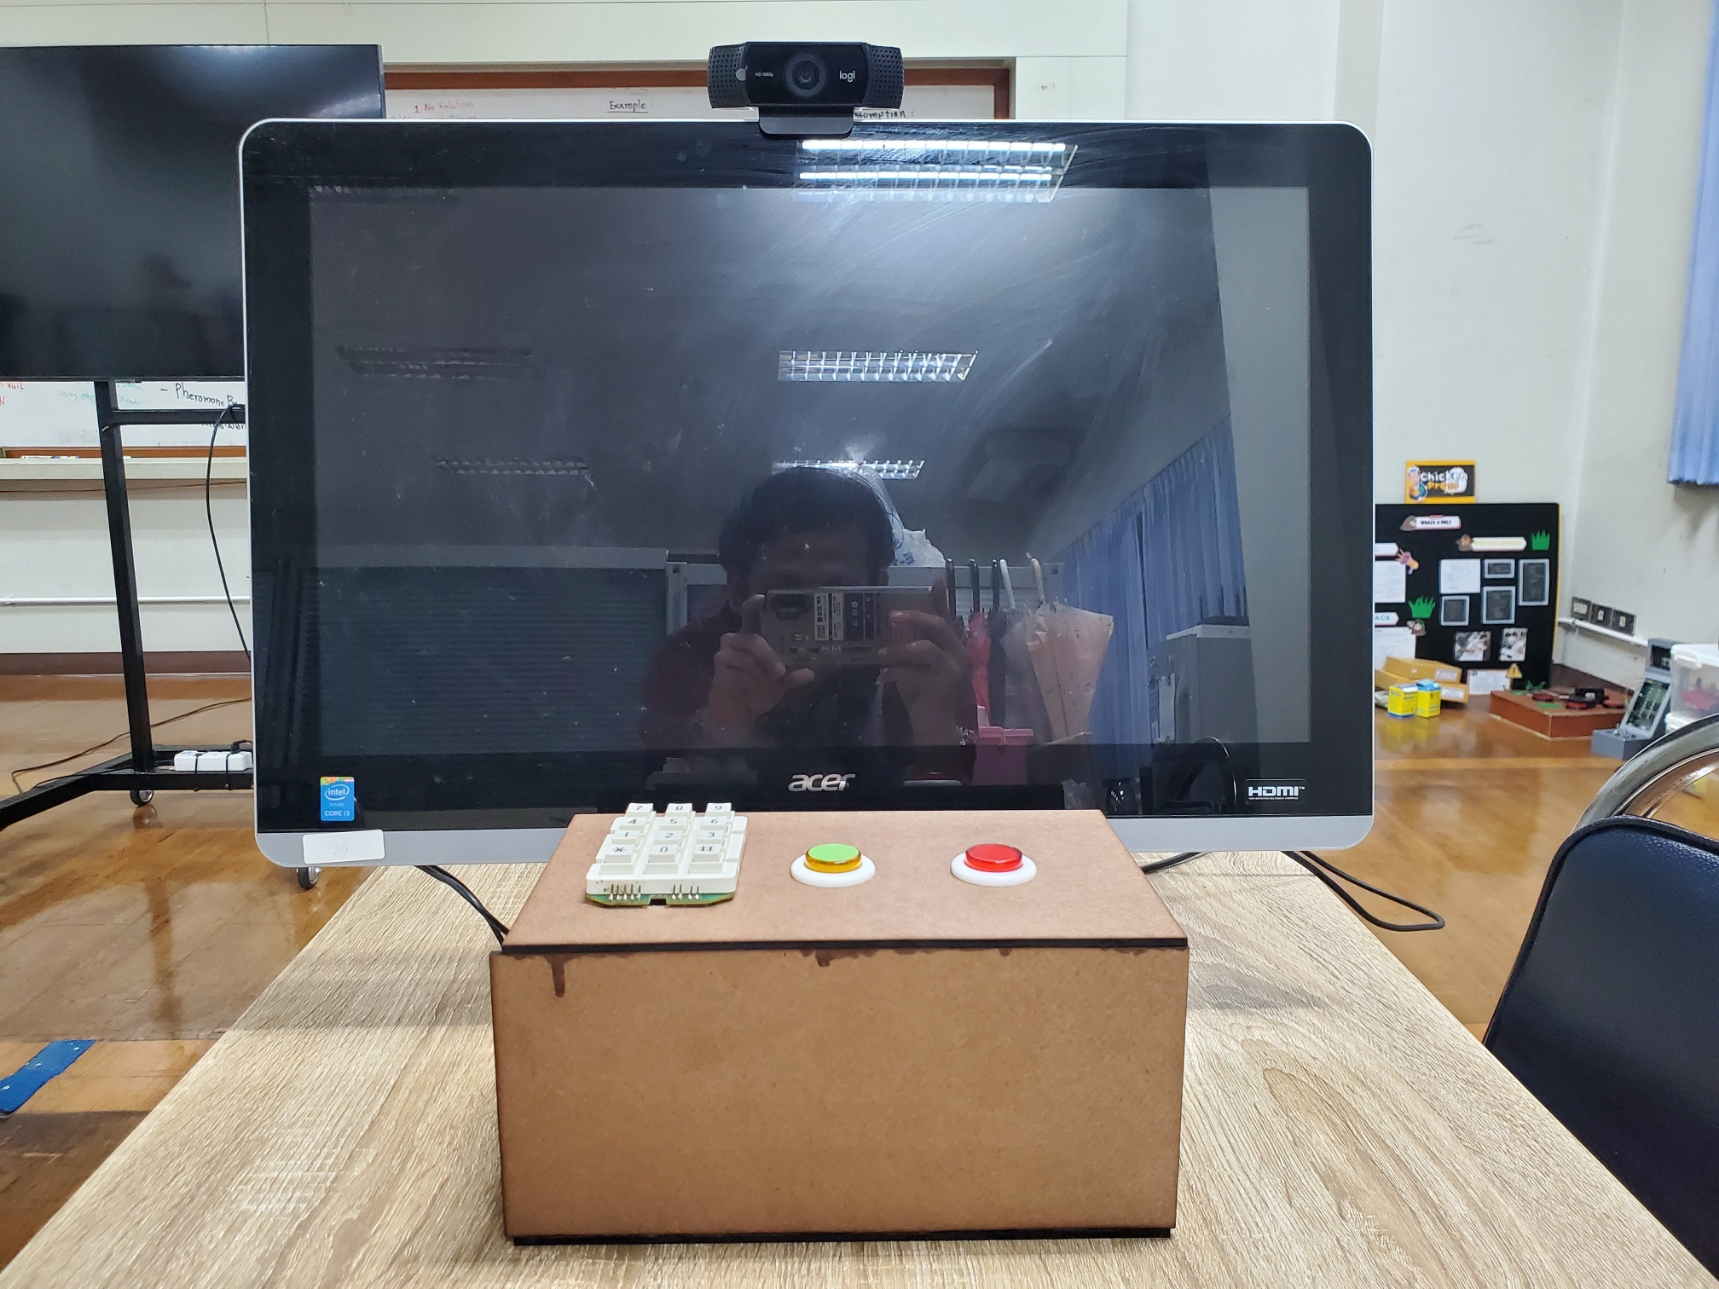
\includegraphics[scale=.1]{pic/system.jpg}
%     \caption[face detection module]{มอดูลที่ใช้ในการระบุตัวตนด้วยรูปภาพใบหน้าและแสดงผล}
%     \label{fig:face_module}
%   \end{center}
% \end{figure}

\begin{figure}[!ht]
  \begin{center}
    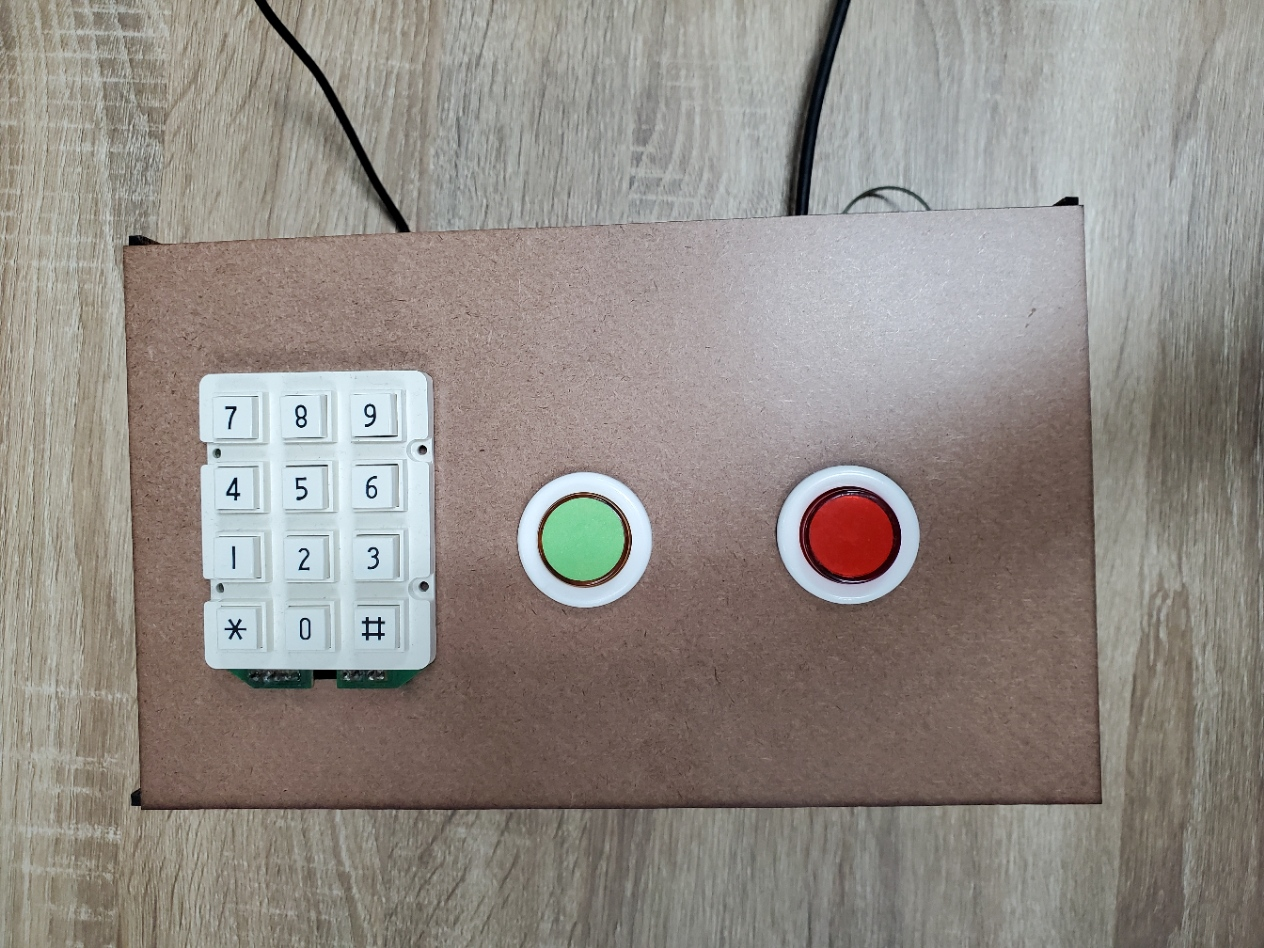
\includegraphics[scale=.17]{pic/rpi_top.jpg}
    \caption[ปุ่มกดให้คะแนนความถูกต้อง]{ปุ่มกดให้คะแนนความถูกต้อง}
    \label{fig:button_module}
  \end{center}
\end{figure}

\begin{figure}[!ht]
  \begin{center}
    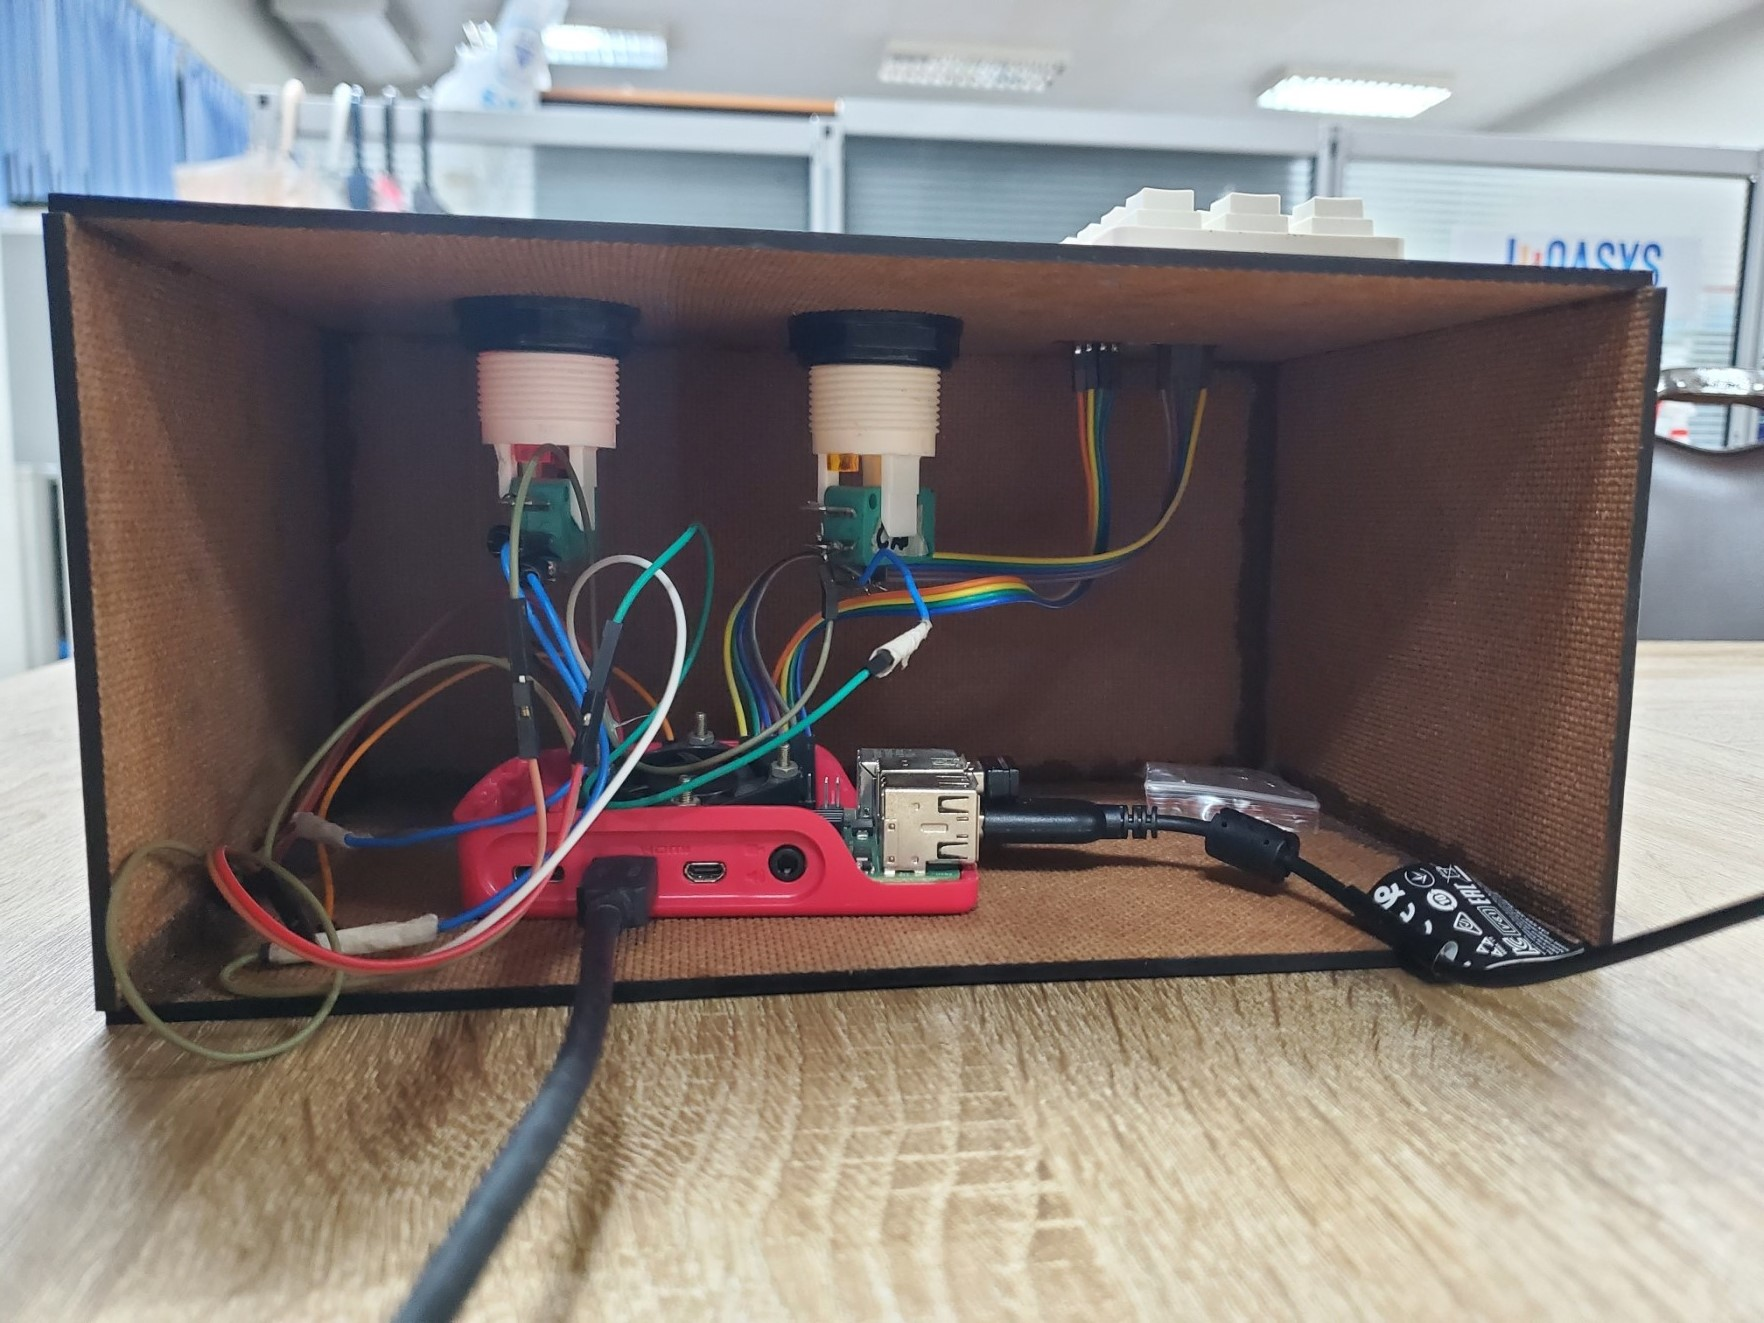
\includegraphics[scale=.17]{pic/rpi_back.jpg}
    \caption[ภายในมอดูลการตรวจจับใบหน้า และแสดงผล]{ภายในมอดูลการตรวจจับใบหน้า และแสดงผล}
    \label{fig:inside_module}
  \end{center}
\end{figure}

\begin{figure}[!ht]
  \begin{center}
    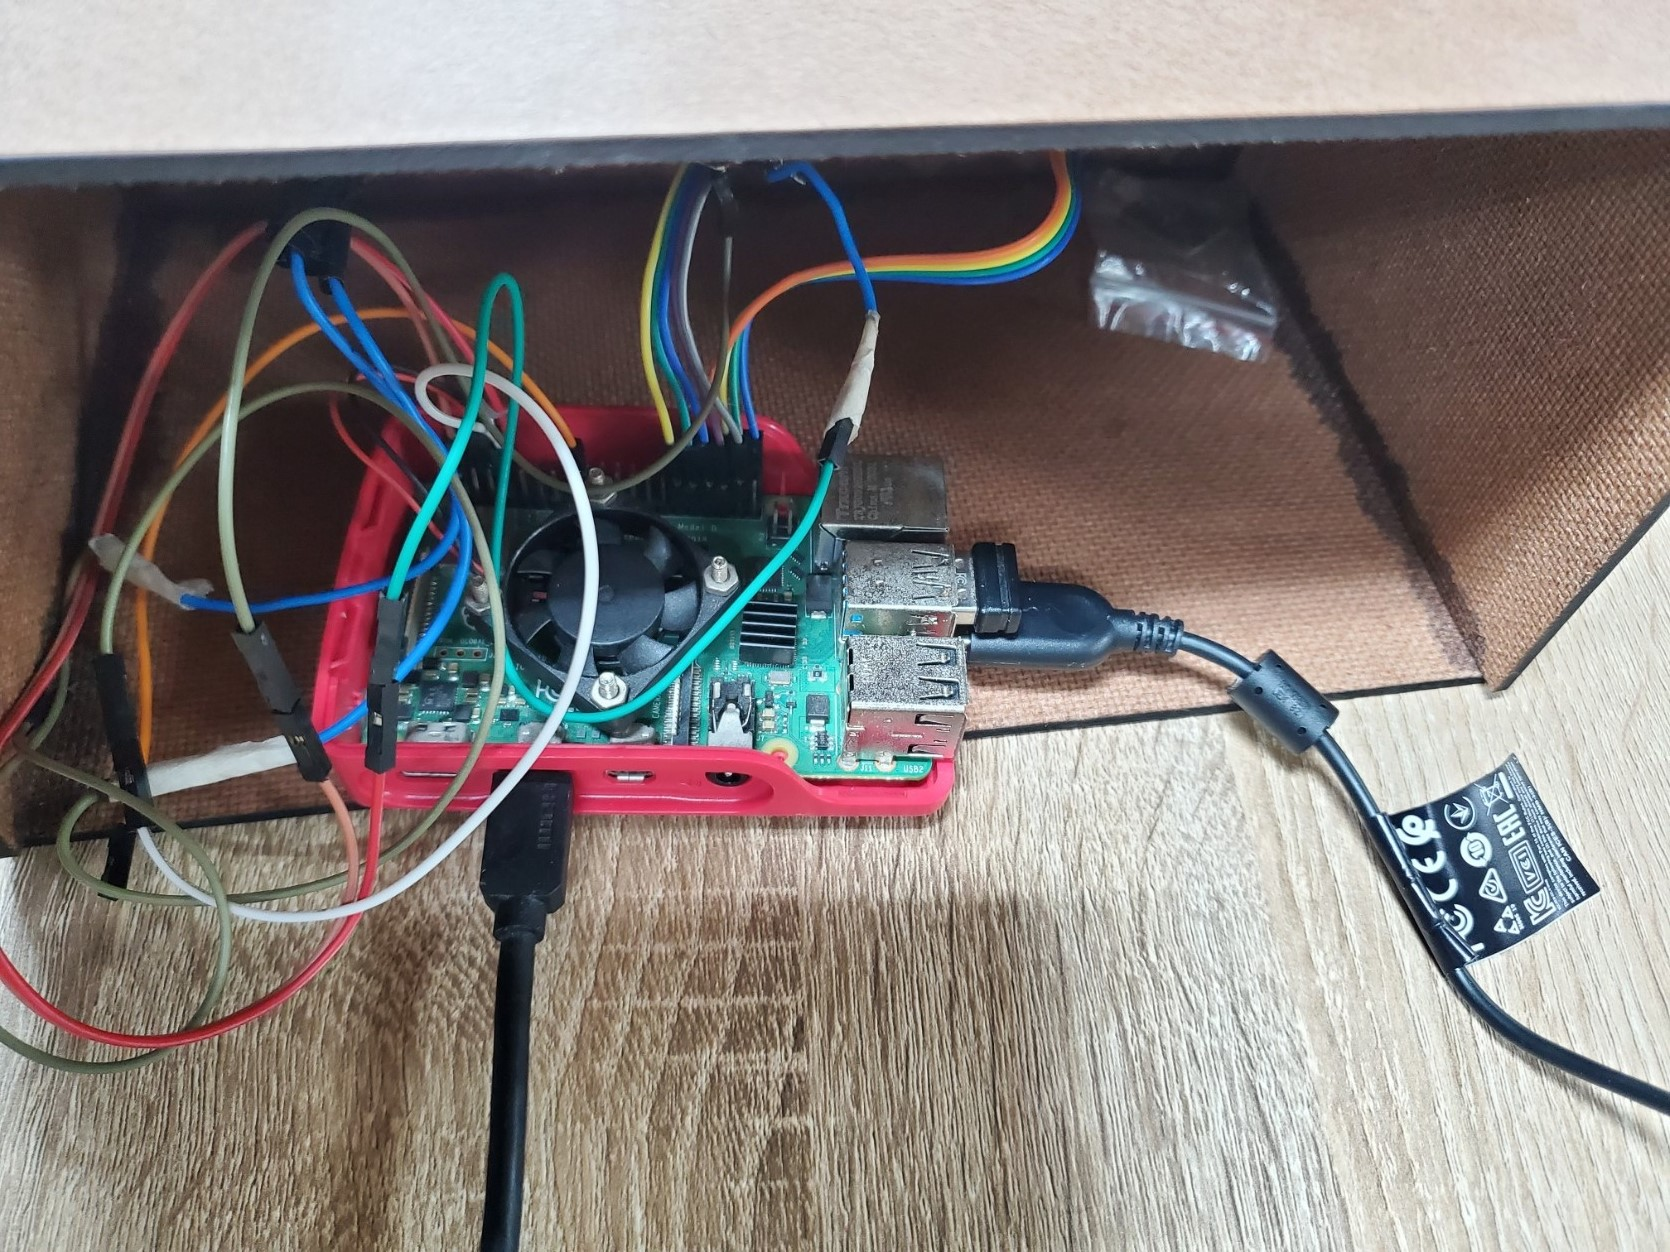
\includegraphics[scale=.17]{pic/rpi.jpg}
    \caption[การเชื่อมต่อ Raspberry Pi]{การเชื่อมต่อ Raspberry Pi}
    \label{fig:rpi_module}
  \end{center}
\end{figure}

\newpage
\section{รูปภาพการแสดงผลบนหน้าจอ}

\begin{figure}[!ht]
    \begin{center}
      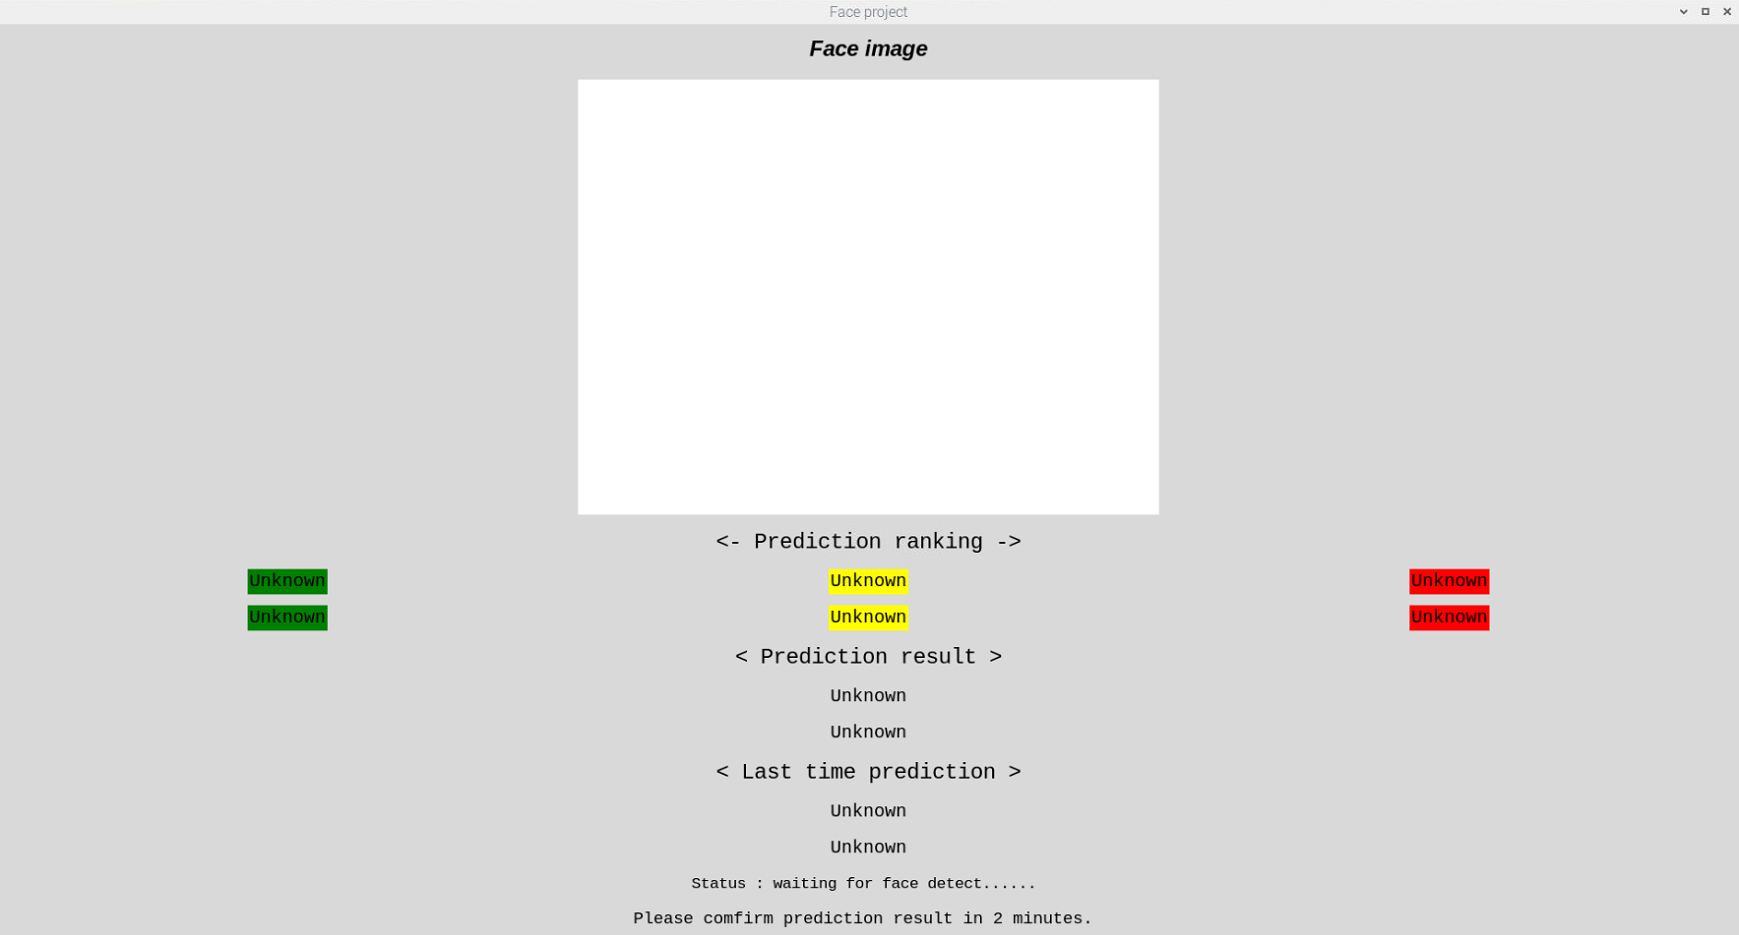
\includegraphics[scale=.35]{pic/main_page.png}
      \caption[หน้า GUI เมื่อโปรแกรมเริ่มทำงาน]{หน้า GUI เมื่อโปรแกรมเริ่มทำงาน}
      \label{fig:main_page}
    \end{center}
  \end{figure}



\begin{figure}[!ht]
    \begin{center}
      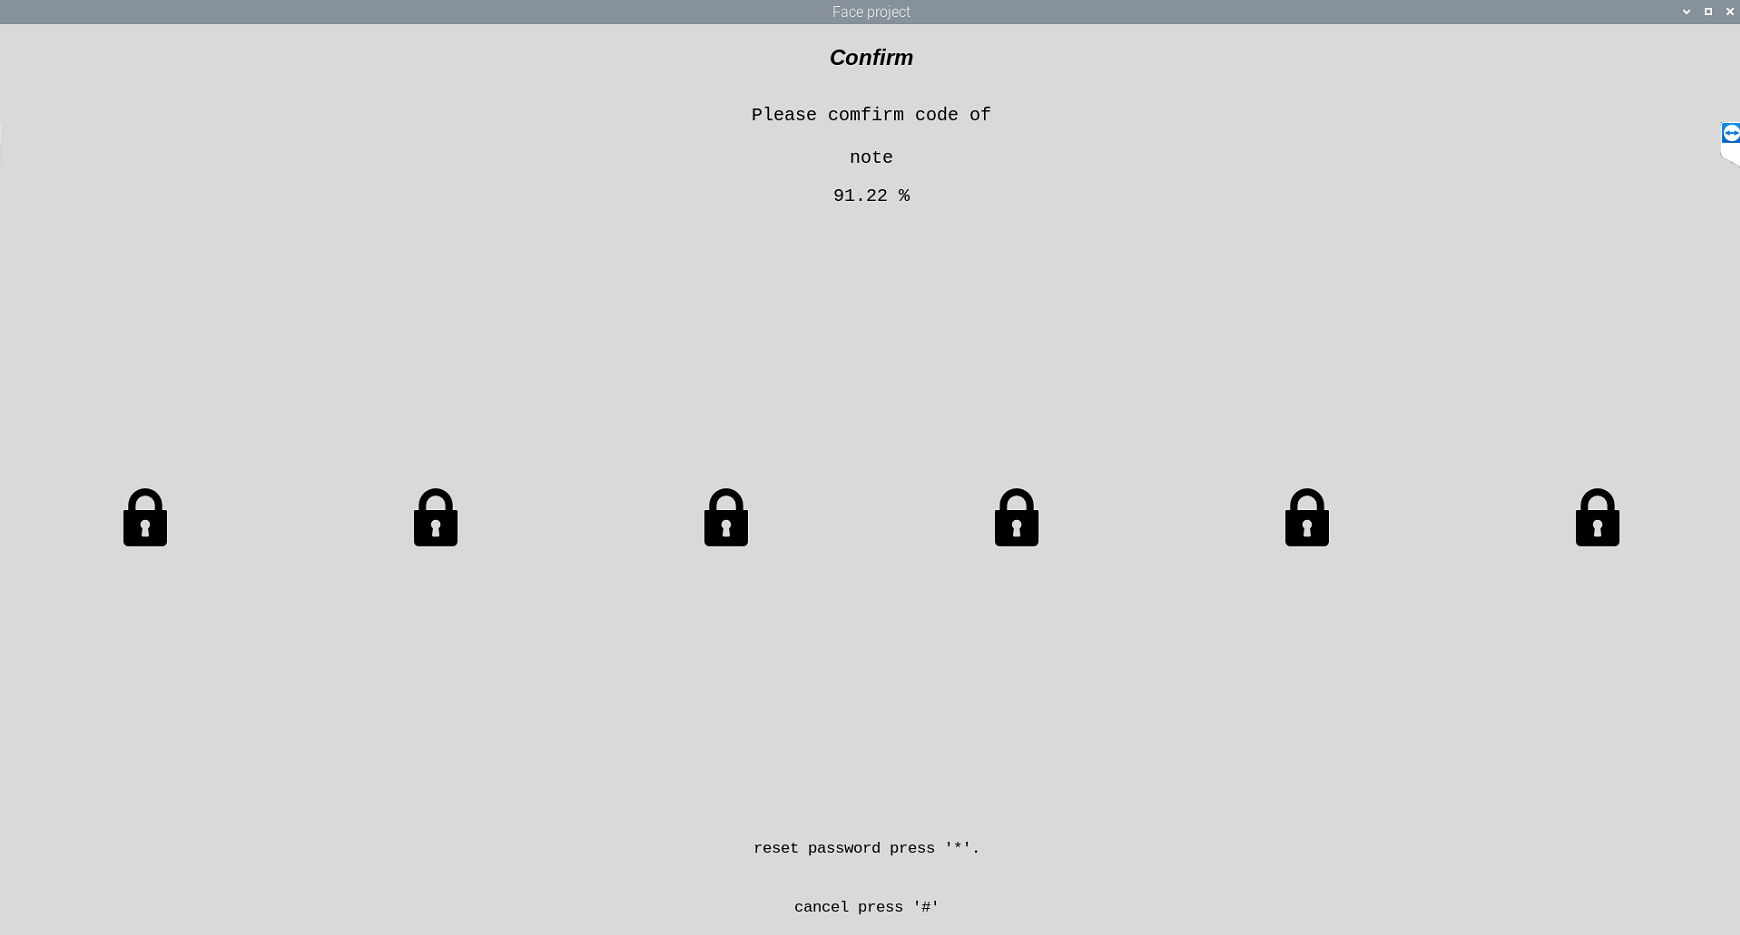
\includegraphics[scale=.35]{pic/comfirm_page.png}
      \caption[หน้า GUI เมื่อผลลัพธ์การระบุตัวตนผิด]{หน้า GUI เมื่อผลลัพธ์การระบุตัวตนผิด}
      \label{fig:com_page}
    \end{center}
  \end{figure}





% \textsf{test ทดสอบฟอนต์ sans serif ภาษาไทย}

% \verb+test ทดสอบฟอนต์ teletype ภาษาไทย+

% \texttt{test ทดสอบฟอนต์ teletype ภาษาไทย}

% \textbf{ตัวหนา serif ภาษาไทย \textsf{sans serif ภาษาไทย} \texttt{teletype ภาษาไทย}}

% \textit{ตัวเอียง serif ภาษาไทย \textsf{sans serif ภาษาไทย} \texttt{teletype ภาษาไทย}}

% \textbf{\textit{ตัวหนาเอียง serif ภาษาไทย \textsf{sans serif ภาษาไทย} \texttt{teletype ภาษาไทย}}}






\chapter{\ifenglish Manual\else คู่มือการใช้งานระบบ\fi}

โปรแกรมของโครงงานนี้สามารถดาวน์โหลดได้จาก \url{https://www.example.com/test_ทดสอบ_url} 
ใช้ระบบปฏิบัติการของ Raspberry Pi คือ Raspbian buster และใช้ระบบปฏิบัติการของ Windows คือ Windows 10

\section{คู่มือการติดตั้งโปรแกรมเพื่อตรวจจับใบหน้าบน Raspberry Pi}
\subsection{คู่มือการติดตั้ง OpenCV บน Raspberry Pi}
\begin{enumerate}
  \item เปิด Termenal
  \item พิมพ์คำสั่ง sudo git clone \url{https://github.com/freedomwebtech/raspbianlegacy.git}
  \item พิมพ์คำสั่ง cd raspbianlegacy
  \item พิมพ์คำสั่ง sudo chmod 775 install.sh
  \item พิมพ์คำสั่ง sudo ./install.sh จากนั้นรอจนกว่าจะเสร็จ ใช้เวลาประมาณ 2 ชั่วโมง
  \item เมื่อทำการติดตั้งเสร็จแล้วให้ทดลองใช้คำสั่ง python3
  \item แล้วพิมพ์ import cv2
  \item แล้วพิมพ์ cv2.\textunderscore\textunderscore version \textunderscore\textunderscore หากติดตั้งสำเร็จจะแสดงเลข version
\end{enumerate}

\subsection{คู่มือการติดตั้ง TensorFlow lite บน Raspberry Pi}
\begin{enumerate}
  \item เปิด Termenal
  \item พิมพ์คำสั่ง sudo git clone \url{https://github.com/freedomwebtech/raspbianlegacy.git}
  \item พิมพ์คำสั่ง cd raspbianlegacy
  \item พิมพ์คำสั่ง sudo chmod 775 tensorflow-lite.sh
  \item พิมพ์คำสั่ง sudo ./tensorflow-lite.sh จากนั้นรอจนกว่าจะเสร็จ
  \item เมื่อทำการติดตั้งเสร็จแล้วให้ทดลองใช้คำสั่ง pip show tensorflow หากติดตั้งสำเร็จจะแสดงข้อมูลของ tensorflow
\end{enumerate}

\subsection{คู่มือการติดตั้ง Mediapipe library บน Raspberry Pi}
\begin{enumerate}
  \item เปิด Termenal
  \item พิมพ์คำสั่ง sudo apt update
  \item พิมพ์คำสั่ง sudo pip3 install mediapipe-rpi4 จากนั้นรอจนกว่าจะเสร็จ
\end{enumerate}

\subsection{คู่มือการติดตั้ง Tkinter library บน Raspberry Pi}
\begin{enumerate}
  \item เปิด Termenal
  \item พิมพ์คำสั่ง sudo apt update
  \item พิมพ์คำสั่ง sudo pip3 install tk จากนั้นรอจนกว่าจะเสร็จ
\end{enumerate}


\section{คู่มือการติดตั้งโปรแกรมเพื่อระบุตัวตนใบหน้าบน Server}
\subsection{คู่มือการติดตั้ง Python บน Windows}
\begin{enumerate}
  \item ไปยังเว็บไซต์ \url{https://www.python.org/downloads/} เพื่อดาวน์โหลดตัว setup ของ Python
  \item เปิดไฟล์ setup
  \item คลิ๊ก Install Now รอจนติดตั้งเสร็จ จากนั้นสามารถกดปิดหน้าต่างการ setup ได้
  \item เมื่อติดตั้ง Python เสร็จแล้ว ให้ทดลองตรวจสอบว่า Python นั้นติดตั้งสําเร็จ โดยการเปิด cmd
  หรือ powershell แล้วใช้คําสั่ง python -V จะแสดง version ของ Python ที่ทําการติดตั้ง
\end{enumerate}

\subsection{คู่มือการติดตั้ง Flask framework}
\begin{enumerate}
  \item เปิด cmd หรือ powershell หรือ windows terminal
  \item พิมพ์คำสั่ง pip install Flask รอจนติดตั้งเสร็จ
\end{enumerate}

\subsection{คู่มือการติดตั้ง OpenCV บน Windows}
\begin{enumerate}
  \item เปิด cmd หรือ powershell หรือ windows terminal
  \item พิมพ์คำสั่ง pip install opencv-python รอจนติดตั้งเสร็จ
  \item เมื่อทำการติดตั้งเสร็จแล้วให้ทดลองใช้คำสั่ง python
  \item แล้วพิมพ์ import cv2
  \item แล้วพิมพ์ cv2.\textunderscore\textunderscore version \textunderscore\textunderscore หากติดตั้งสำเร็จจะแสดงเลข version
\end{enumerate}

\subsection{คู่มือการติดตั้ง Scikit learn บน Windows}
\begin{enumerate}
  \item เปิด cmd หรือ powershell หรือ windows terminal
  \item พิมพ์คำสั่ง pip install scikit-learn รอจนติดตั้งเสร็จ
\end{enumerate}


\section{คู่มือการใช้งานการตรวจจับใบหน้า}
\begin{enumerate}
  \item เปิด Termenal
  \item พิมพ์คำสั่ง git clone \url{https://github.com/freedomwebtech/raspbianlegacy.git}
  \item หลังจากนั้นพิมพ์คำสั่ง cd face derection
  \item เปิดไฟล์ request\textunderscore response.py 
  \item แก้ url ให้เป็นเลข IP Address ของ server รับรูปภาพ
  \item พิมพ์คำสั่ง python main\textunderscore ui.py
\end{enumerate}

หลังจากพิมพ์คำสั่ง python main\textunderscore ui.py จะแสดงหน้าตา UI ดังรูป

\begin{figure}[!ht]
  \begin{center}
    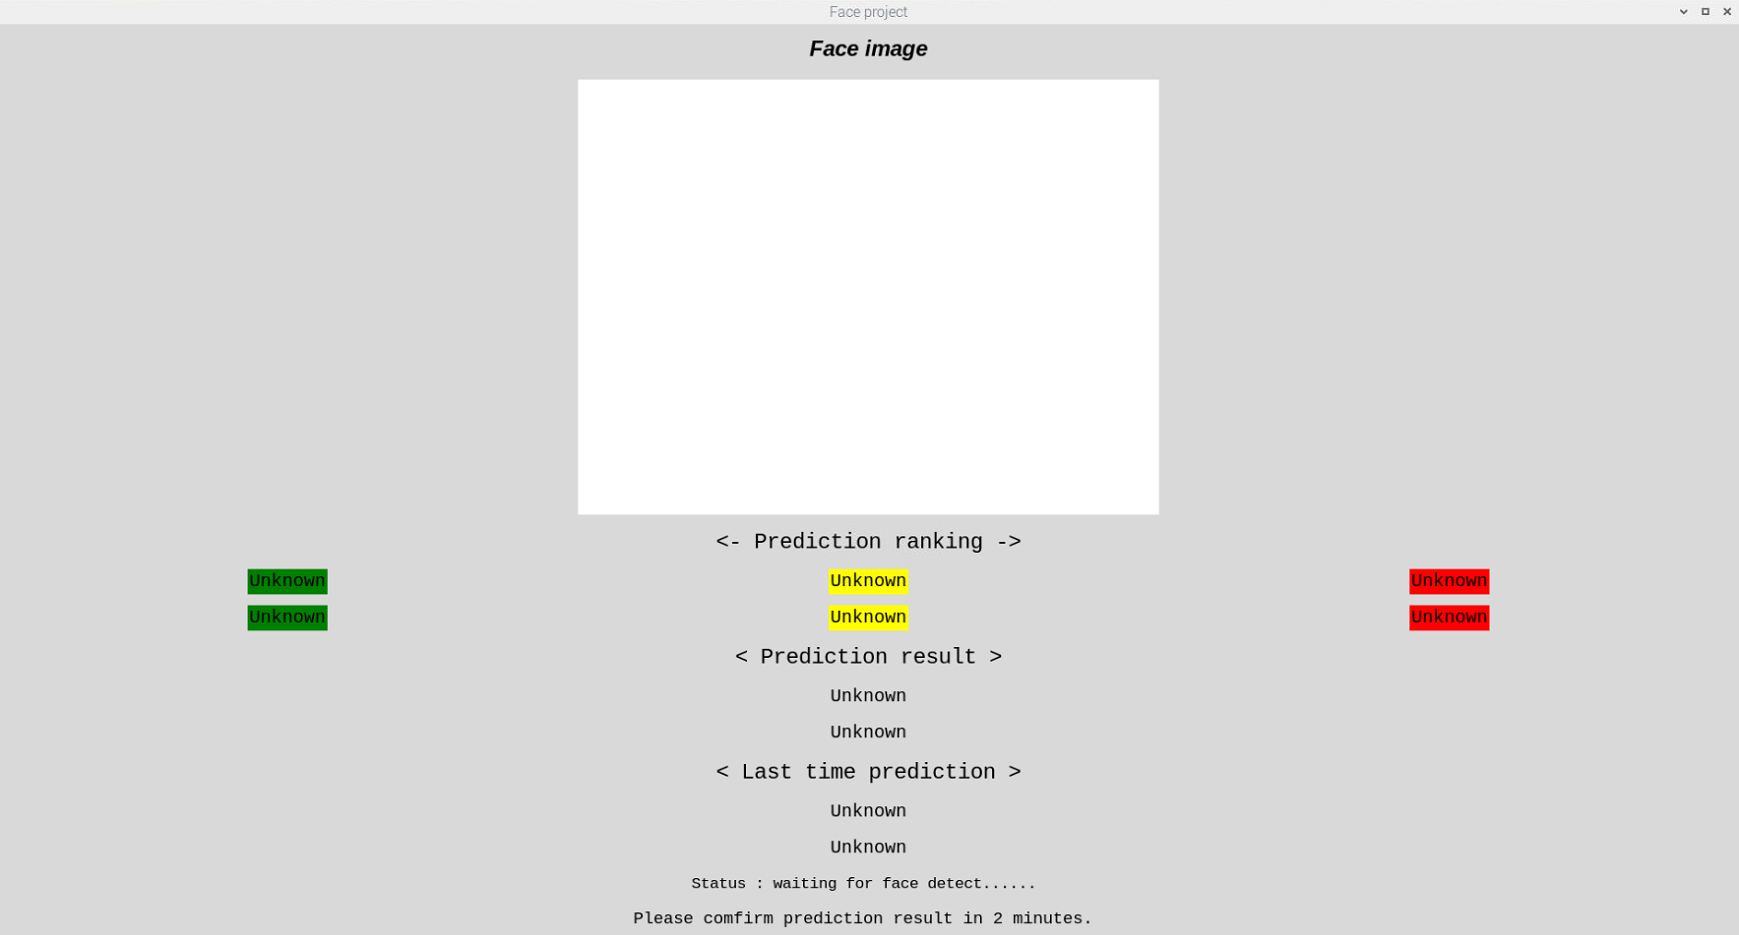
\includegraphics[scale=.3]{pic/main_page.png}
    \caption{หน้า GUI เมื่อโปรแกรมเริ่มทำงาน}
  \end{center}
\end{figure}

\section{คู่มือการใช้งานการระบุตัวตนด้วยใบหน้า}
\begin{enumerate}
  \item เปิด cmd หรือ powershell หรือ windows terminal
  \item พิมพ์คำสั่ง git clone \url{https://github.com/protonnote/backend-graduate-project.git}
  \item หลังจากนั้นพิมพ์คำสั่ง cd backend-graduate-project
  \item หลังจากนั้นเปิดไฟล์ app.py เพื่อแก้ที่จัดเก็บรูปภาพ (UPLOAD\textunderscore FOLDER) ตามเส้นทาง (path) ที่อยู่ปัจจุบันให้ถูกต้องแล้วบันทึก
  \item พิมพ์คำสั่ง python main.py
\end{enumerate}

หลังจากพิมพ์คำสั่ง python main.py จะแสดงหน้าตา Termenal ดังรูป
\begin{figure}[!ht]
  \begin{center}
    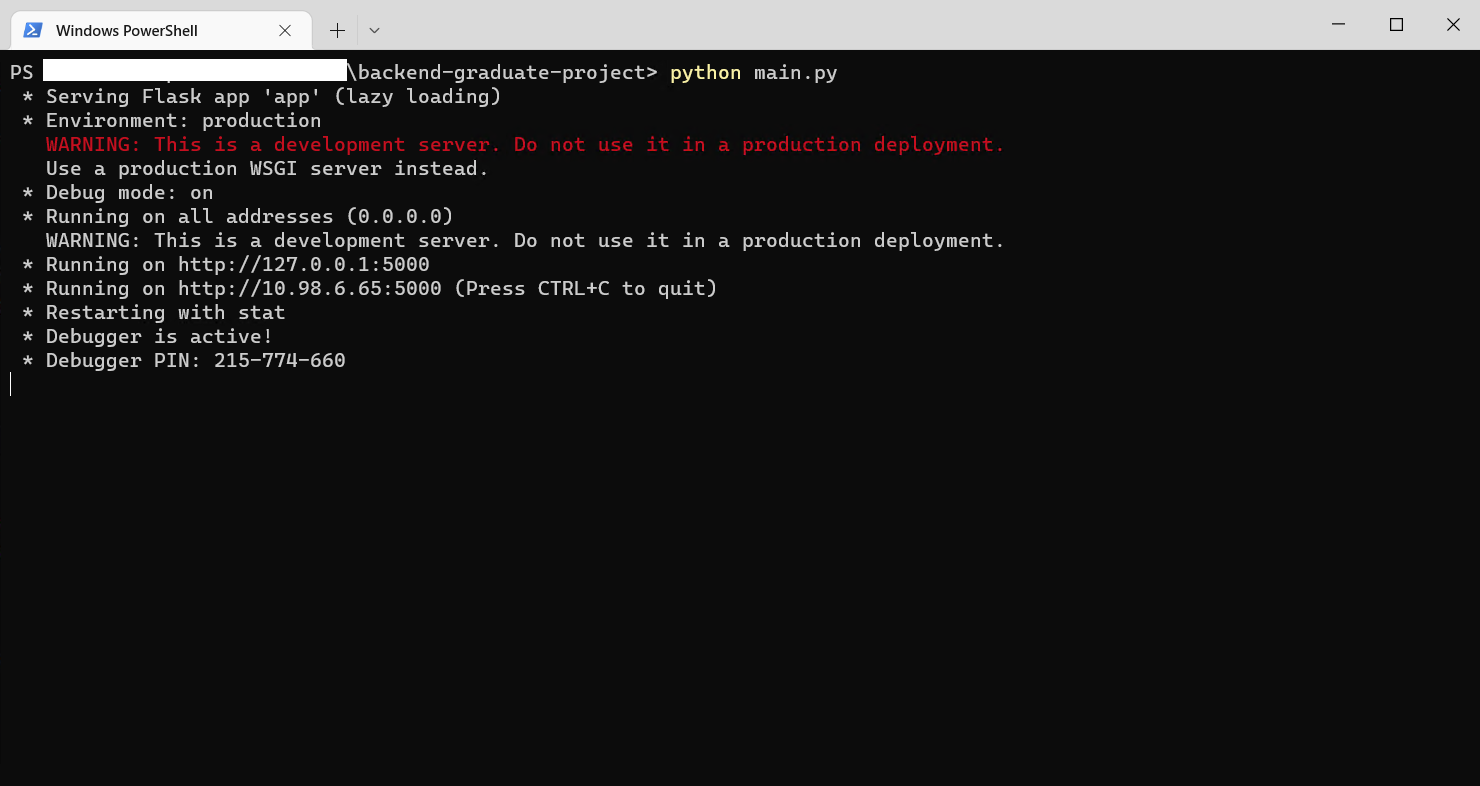
\includegraphics[scale=.4]{pic/server_start.png}
    \caption[หน้า Terminal เมื่อโปรแกรมระบุตัวตนด้วยใบหน้าเริ่มทำงาน]{หน้า Terminal เมื่อโปรแกรมระบุตัวตนด้วยใบหน้าเริ่มทำงาน}
    \label{fig:server_start}
  \end{center}
\end{figure}